\documentclass[conference]{IEEEtran}
\IEEEoverridecommandlockouts

\usepackage{cite}
\usepackage{amsmath,amssymb,amsfonts}
\usepackage{algorithmic}
\usepackage{graphicx}
\usepackage{textcomp}
\usepackage{xcolor}
\usepackage{textcomp}
\usepackage{float}
\usepackage{array}
\usepackage{siunitx}
\usepackage{tabularx}
\usepackage{listings}
\usepackage[colorlinks=false]{hyperref}
\def\BibTeX{{\rm B\kern-.05em{\sc i\kern-.025em b}\kern-.08em
    T\kern-.1667em\lower.7ex\hbox{E}\kern-.125emX}}

\setlength{\parindent}{0pt}

% Define the custom column type Y
\newcolumntype{Y}{>{\centering\arraybackslash} m{1.9cm}}

\definecolor{codeblue}{rgb}{0.2,0.2,0.6}
\definecolor{codegreen}{rgb}{0.133,0.545,0.133}
\definecolor{codegray}{rgb}{0.5,0.5,0.5}
\definecolor{codepurple}{rgb}{0.58,0,0.82}
\definecolor{backcolour}{rgb}{0.95,0.95,0.92}

\lstdefinestyle{mystyle}{
    backgroundcolor=\color{backcolour},
    commentstyle=\color{codegreen},
    keywordstyle=\color{codeblue},
    numberstyle=\tiny\color{codegray},
    stringstyle=\color{codepurple},
    basicstyle=\ttfamily\scriptsize,
    breakatwhitespace=false,
    breaklines=true,
    captionpos=b,
    keepspaces=true,
    numbers=none,
    numbersep=5pt,
    showspaces=false,
    showstringspaces=false,
    showtabs=false,
    tabsize=2
}

\lstset{style=mystyle}

\begin{document}

\title{Robotics and Mechatronics\\
{\LARGE Homework One}
}

\author{\IEEEauthorblockN{Mohammad Montazeri}
\IEEEauthorblockA{\textit{School of Mechanical Engineering} \\
\textit{College of Engineering, University of Tehran}\\
Tehran, Iran \\
mohammadmontazeri@ut.ac.ir}
}

\maketitle

\begin{abstract}
In this Homework, we first learn and practice the basics of the Robotics course. 
\end{abstract}

\begin{IEEEkeywords}
Robots, Linear invariants, Quadratic invariants, Euler-Rodrigues Parameters, Rotation matrix, Transformation
\end{IEEEkeywords}

\section{Introduction}
The field of robotics encompasses a wide range of concepts and principles that are crucial for understanding the design, control, and operation of robotic systems. This Homework discusses mainly about the basics of Robotics-Mechatronics course lectured in the first 3 chapters of the textbook \cite{b1}. In this report, we will delve into various topics related to fixed-based robots, mobile-based robots, mechanical joints, mathematical background, and rotational transformations. Through a series of problems, we will explore key concepts such as yaw, pitch, roll, Plücker lines, rotation matrices, and the properties of rotation matrices. Each problem is designed to deepen our understanding of these fundamental principles and their applications in robotics. 

\vspace{5px}
\section{Problem 1: Fixed-based Robots}
\subsection{Serial Robots}
Serial robots, also known as serial manipulators, consist of a chain of interconnected links and joints. They form a sequential structure where each joint depends on the previous one.
\begin{itemize}
    \item Advantages:
    \begin{enumerate}
        \item Simplicity: Serial robots are conceptually simpler due to their linear structure.
        \item Workspace Flexibility: They can reach a wide range of positions within their workspace.
        \item Cost-Effectiveness: Generally, serial robots are more cost-effective to manufacture and maintain.
        \item Ease of Programming: Their programming is straightforward, making them suitable for various applications.
    \end{enumerate}
    \item Disadvantages:
    \begin{enumerate}
        \item Limited Stiffness: Serial robots exhibit lower stiffness, affecting their precision and accuracy.
        \item Inertia Accumulation: The inertia of each link accumulates, leading to reduced dynamic performance.
        \item Complex Inverse Kinematics: Solving inverse kinematics can be challenging for complex serial structures.
    \end{enumerate}
\end{itemize}

\subsection{Parallel Robots}
Parallel robots, also called parallel manipulators, feature multiple limbs connected to a common platform or end effector. These limbs move simultaneously.
\begin{itemize}
    \item Advantages:
    \begin{enumerate}
        \item High Stiffness: Parallel robots offer superior stiffness, enhancing precision and stability.
        \item Increased Acceleration: They achieve faster accelerations and decelerations.
        \item Reduced Inertia: The inertia of individual limbs does not accumulate, improving dynamic performance.
        \item Enhanced Accuracy: Parallel robots excel in applications requiring high accuracy.
    \end{enumerate}
    \item Disadvantages:
    \begin{enumerate}
        \item Complex Design: Their structural complexity can make manufacturing and maintenance challenging.
        \item Limited Workspace: Parallel robots often have a smaller workspace compared to serial robots.
        \item Higher Cost: Due to their intricate design, parallel robots can be costlier.
        \item Kinematic Singularities: Certain configurations may encounter singularities, affecting motion.
    \end{enumerate}
\end{itemize}

In summary, serial robots are simpler and versatile, while parallel robots offer better stiffness and precision. The choice depends on specific application requirements and trade-offs between simplicity, workspace, and performance \cite{b2}\cite{b3}\cite{b4}. 

\vspace{10px}
\section{Problem 2: Mobile-based Robots}
\subsection*{Part 1)}
Nao is an autonomous, programmable humanoid robot formerly developed by Aldebaran Robotics, a French robotics company headquartered in Paris, which was acquired by SoftBank Group in 2015 and rebranded as SoftBank Robotics. The robot's development began with the launch of Project Nao in 2004 \cite{b5}. Some of its most astonishing features are \cite{b6}\cite{b7}:

\begin{enumerate}
    \item \textbf{ultilingual Communication}: Nao is fluent in more than 20 languages, allowing it to communicate clearly and effortlessly with students from diverse cultural backgrounds.
    \item \textbf{Tactile Sensing and Interaction}: Nao can feel its environment due to tactile sensors in its head, hands, and feet. These sensors enable Nao to react and respond appropriately, enhancing its interaction with humans. Whether it's recognizing touch or avoiding obstacles, Nao's tactile awareness contributes to its versatility.
    \item \textbf{Agile Movement and Navigation}: Standing at approximately 58 cm (22.8 inches) in height, Nao is a bipedal robot with pleasantly rounded features. It is built to move naturally and can go almost anywhere. Nao can detect obstacles, avoid falls, and quickly recover if it stumbles.
    \item \textbf{Programmability and Customization}: Nao runs on \textit{NAOqi OS}, a flexible framework that allows extensive customization. Developers can program Nao using various tools, including SDKs, visual programming interfaces like Blockly and Scratch, and Choregraphe, an easy-to-use drag-and-drop graphical software. This openness empowers educators and researchers to tailor Nao's behavior and capabilities to their specific needs.
    \item \textbf{Research and Experimentation}: Researchers use Nao to conduct experiments, collect data, and test theories. Its ability to interact with people on a personal level makes it valuable for various research domains.
\end{enumerate}


In summary, Nao's combination of language skills, environmental awareness, mobility, programmability, and friendly demeanor contributes to its utility and versatility across diverse robotics applications in the classroom, the lab, or healthcare settings \cite{b8}.

\subsection*{Part 2)}
According to the provider company, Aldebaran, a part of United Robotics Group, Nao \textsuperscript{6} has 25 degrees of freedom which enable him to move and adapt to his environment.

\subsection*{Part 3)}
The \textit{Nao humanoid robot}, developed by \textit{SoftBank Robotics}, combines both \underline{series} and \underline{parallel joint configurations} to enhance its functionality \cite{b9}. Here we explore these joint types and discuss their advantages and applications in robotics:

\subsubsection*{A. Series Joints (Serial Kinematics)}

\begin{enumerate}
    \item \textbf{Definition}:
        \begin{itemize}
            \item Series joints form a \textbf{sequential chain} where each joint depends on the previous one.
            \item In Nao, series joints are used for the arms, legs, and neck.
        \end{itemize}
    \item \textbf{Advantages}:
        \begin{itemize}
            \item \textbf{Simplicity}: Series joints are conceptually simpler due to their linear structure.
            \item \textbf{Workspace Flexibility}: They can reach a wide range of positions within their workspace.
            \item \textbf{Cost-Effectiveness}: Generally, series joints are more cost-effective to manufacture and maintain.
            \item \textbf{Ease of Programming}: Their programming is straightforward.
        \end{itemize}
    \item \textbf{Disadvantages}:
        \begin{itemize}
            \item \textbf{Limited Stiffness}: Series joints exhibit lower stiffness, affecting precision and accuracy.
            \item \textbf{Inertia Accumulation}: The inertia of each link accumulates, leading to reduced dynamic performance.
            \item \textbf{Complex Inverse Kinematics}: Solving inverse kinematics can be challenging for complex serial structures.
        \end{itemize}
\end{enumerate}

\subsubsection*{B. Parallel Joints (Parallel Kinematics)}

\begin{enumerate}
    \item \textbf{Definition}:
        \begin{itemize}
            \item Parallel joints feature multiple limbs connected to a common platform or end effector.
            \item In Nao, parallel joints are used for the head and hands.
        \end{itemize}
    \item \textbf{Advantages}:
        \begin{itemize}
            \item \textbf{High Stiffness}: Parallel joints offer superior stiffness, enhancing precision and stability.
            \item \textbf{Increased Acceleration}: They achieve faster accelerations and decelerations.
            \item \textbf{Reduced Inertia}: The inertia of individual limbs does not accumulate, improving dynamic performance.
            \item \textbf{Enhanced Accuracy}: Parallel joints excel in applications requiring high accuracy.
        \end{itemize}
    \item \textbf{Disadvantages}:
        \begin{itemize}
            \item \textbf{Complex Design}: Their structural complexity can make manufacturing and maintenance challenging.
            \item \textbf{Limited Workspace}: Parallel joints often have a smaller workspace compared to series joints.
            \item \textbf{Higher Cost}: Due to their intricate design, parallel joints can be costlier.
            \item \textbf{Kinematic Singularities}: Certain configurations may encounter singularities, affecting motion.
        \end{itemize}
\end{enumerate}

\subsubsection*{C. Applications in Nao}
\begin{itemize}
    \item \textbf{Series Joints (Arms and Legs)}:
        \begin{itemize}
            \item Precise arm movements for grasping objects.
            \item Natural leg motion for walking and dynamic locomotion.
        \end{itemize}
    \item \textbf{Parallel Joints (Head and Hands)}:
        \begin{itemize}
            \item High stiffness in the head for stable vision and interaction.
            \item Dexterity in the hands for fine manipulation (e.g., picking up objects).
        \end{itemize}
\end{itemize}

In summary, Nao's combination of series and parallel joints allows it to perform a wide range of tasks, from walking and grasping to expressive head movements. The choice of joint type depends on specific requirements and trade-offs between simplicity, workspace, and performance \cite{b10}.

\section{Problem 3: Mechanical joints}
In the provided video, multiple types of joints found in a human body are mentioned, such as:
\begin{itemize}
    \item \textbf{Synovial joint}: A synovial joint is the type of joint found between bones that move against each other, such as the joints of the limbs (e.g. shoulder, hip, elbow and knee). Characteristically it has a joint cavity filled with fluid.
    \item \textbf{Fibrous joints}: Fibrous joints are defined as the joints in which the bones are connected by fibrous tissue. They are called fixed or immovable joints as they do not allow any movement between the bones.
    \item \textbf{Cartilaginous joints}: Cartilaginous joints are a type of joint where the bones are entirely joined by cartilage, either hyaline cartilage or fibrocartilage. These joints generally allow more movement than fibrous joints but less movement than synovial joints.
\end{itemize}

The more usually used and practical joints in robotics are like \textit{Synovial joints} mentioned in the video, which consist of a variety of kinds listed as below \cite{b11}. 
\begin{enumerate}
    \item Hinge
    \item Pivot
    \item Ball and Socket
    \item Ellipsoid
    \item Saddle
    \item Plane
\end{enumerate}

Here we explore their mechanical equivalent and explain the similarity behind them [Table \ref{tab:table_one}][Table \ref{tab:table_two}].
{
\setlength{\tabcolsep}{4pt} % Adjust the padding for this specific table
\renewcommand{\arraystretch}{1.5} % Default value is 1

\begin{table}[htbp]
    \caption{Types of joints found in human body and their mechanical equivalent}
    \begin{center}
        \begin{tabular}{|Y|Y|m{110px}|}
            \hline
            Anatomical joint & Mechanical joint & Description \\
            \hline
            Hinge & Pin/Revolute & A pin joint, also called a revolute joint, is a one-degree-of-freedom kinematic pair. It constrains the motion of two bodies to pure rotation along a common axis. The joint doesn't allow translation, or sliding linear motion. This is usually done through a rotary bearing. It enforces a cylindrical contact area, which makes it a lower kinematic pair, also called a full joint.\\
            \hline
            Pivot & Cylindrical/Pin & Like Hinge joints, Pivot joints are also 1-DOF joints that allow rotation about one axis. However, if we consider that Pivot joints might slightly alow axial translation, the might be modeled as a combination of Pin and Prismatic (slider) joint.\\
            \hline
            Ball \& socket & Spherical/Ball & A ball joint, as a 3-DOF joint, consists of a bearing stud and socket enclosed in a casing; all these parts are made of steel. The bearing stud is tapered and threaded, and fits into a tapered hole in the steering knuckle. A ball joint is used for allowing free rotation in two planes at the same time while preventing translation in any direction, including rotating in those planes. Combining two such joints with control arms enables motion in all three planes, allowing the front end of an automobile to be steered and a spring and shock (damper) suspension to make the ride comfortable.\\
            \hline
            Ellipsoid & Condyloid & Ellipsoid joint is a restricted kind of Ball and Socket joint. Ellipsoids just have more of an egg shape rather than ball shape. That prevents them from having rotation in all 3 planes. So they're known as 2-DOF joint. Condyloid or condylar joints are another name for this. It is an ovoid articular surface or condyle that receives an elliptical cavity. This allows for two-plane movement, including flexion, extension, adduction, abduction, and circumduction.\\
            \hline
            Saddle & Universal & A universal joint (also called a universal coupling or U-joint) is a joint or coupling connecting rigid shafts whose axes are inclined to each other. It is commonly used in shafts that transmit rotary motion. It consists of a pair of hinges located close together, oriented at 90 to each other, connected by a cross shaft. The universal joint is not a constant-velocity joint. It must be noted that U-joints are also 2-DOF joints that allow rotation in two planes.\\
            \hline
        \end{tabular}
    \end{center}
    \label{tab:table_one}
\end{table}


\begin{table}[htbp]
    \caption{Resume of table 1}
    \centering
    \begin{tabular}{|Y|Y|m{120px}|}
        \hline
        Anatomical joint & Mechanical joint & Description \\
        \hline
        Plane & Planar/Prismatic & Planar joints have bones with articulating surfaces that are flat or slightly curved faces. These joints allow for gliding movements, and so the joints are sometimes referred to as gliding joints. The range of motion is limited in these joints and does not involve rotation. Planar joints are found in the carpal bones in the hand and the tarsal bones of the foot, as well as between vertebrae. A prismatic joint is a basically a 1-DOF kinematic pair which constrains the motion of two bodies to sliding along a common axis, without rotation; for this reason it is often called a slider (as in the slider-crank linkage) or a sliding pair. A combination of prismatic joints can enable translation in more than one plane. A pin joint assembled on top of a prismatic joint might enable rotating additionally. With respect to the case of use, a planar joint can be modeled as a prismatic joint in mechanics.\\
        \hline
    \end{tabular}
    \label{tab:table_two}
\end{table}
}

\vspace{10px}
\section{Problem 4: Mathematical background}
\subsection*{Part 1)}
Let \( \mathbf{w} \) be perpendicular to \( \mathbf{v} \) (\( \mathbf{w}^T\mathbf{v} = \mathbf{v}^T\mathbf{w} = 0 \)). Since we can find two such vectors, let us call them \( \mathbf{w}_1 \) and \( \mathbf{w}_2 \), which lie in the plane normal to \( \mathbf{v} \), but are otherwise arbitrary—no need to assume that these two vectors are mutually orthogonal. We then have
\[
\mathbf{T} = \mathbf{I} + \mathbf{u}\mathbf{v}^T
\]
Multiplying both sides by \( \mathbf{w}_i \), we obtain
\[
\mathbf{T}\mathbf{w}_i = \mathbf{w}_i + \mathbf{u}\mathbf{v}^T\mathbf{w}_i = \mathbf{w}_i,  \quad i=1,2 
\]
Therefore, \( \text{w}_1 \) and \( \textbf{w}_2 \) are eigenvectors of \text{T}, of eigenvalues \( \lambda_1 =  \lambda_2 = 1.\)

Moreover, let 
\[ 
\mathbf{w}_3 = 	\frac{\mathbf{u}}{||\mathbf{u}||} 
\]
Then,
\[
\mathbf{T}\mathbf{w}_3=	\mathbf{w}_3+\mathbf{u}\mathbf{v}^T\mathbf{w}_3=		\underbrace{\frac{\mathbf{u}}{||\mathbf{u}||}}_{\mathbf{w}_{3}}+\mathbf{v}^{T}\mathbf{u}\underbrace{\frac{\mathbf{u}}{||\mathbf{u}||}}_{\mathbf{w}_{3}}
=\left(1+\mathbf{v}^{T}\mathbf{u}\right)\underbrace{\frac{\mathbf{u}}{||\mathbf{u}||}}_{\mathbf{w}_{3}} \rightarrow
\]

\[
\mathbf{T}\mathbf{w}_3 = \left(1+\mathbf{v}^{T} \mathbf{u}\right)\mathbf{w}_{3}
\]


and \(\mathbf{w}_{3}\) is the third eigenvector of T, of eigenvalue \(\underbrace{\lambda}_{3}=1+\mathbf{v}^{T} \mathbf{u}.\)
\subsection*{Part 2)}
The determinant of a matrix is equal to the product of its eigenvalues. Thus
\[
\det(1 + \mathbf{u}\mathbf{v}^T) = \det(\mathbf{T}) = \lambda_1\lambda_2\lambda_3 = 1 + \mathbf{v}^T\mathbf{u} = 1 + u \cdot v.
\]
This can also be experimentally proved by defining two general and parametric vectors \( \mathbf{u} and \mathbf{v} \) in python and find the values of the two sides of the target equation. This is done by the \underline{Python} code attached to this file and also in appendix. Here's the result of this code:
\scriptsize
\begin{verbatim}
    Vector U: [[u0], [u1], [u2]]
    Vector V: [[v0], [v1], [v2]]
    Left Hand Side of the equation:  
        1.0*u0*v0 + 1.0*u1*v1 + 1.0*u2*v2 + 1.0
    Right Hand Side of the equation:         
        [[u0*v0 + u1*v1 + u2*v2 + 1]]
    The difference of LHS and RHS of the equation:   
        [[0]]
\end{verbatim}

\vspace{10px}
\section{Problem 5: Yaw, pitch and roll}
From the reference text book \cite{b12}, the rotation matrix for a fixed origin system that implies to rotating $\gamma$ degrees about $x$, $\beta$ degrees about $y$, and $\alpha$ degrees about $z$ axes is introduced as below. Note that with this deceleration, $\gamma$, $\beta$ and $\alpha$ imply to \textbf{Roll}, \textbf{Pitch} and \textbf{Yaw} respectively.
$$
R_{xyz}(\gamma, \beta, \alpha) = 
\begin{bmatrix}
    c\alpha c\beta & c\alpha s\beta s\gamma - s\alpha c\gamma & c\alpha s\beta c\gamma + s\alpha s\gamma \\
    s\alpha c\beta & s\alpha s\beta s \gamma + c \alpha  c \gamma & s \alpha s \beta c \gamma -	c \alpha s \gamma \\
    -s\beta & c \beta s \gamma & c \beta c\gamma
\end{bmatrix}
$$
The numerical value of this rotation matrix is given as:

{\large
$$
\mathbf{Q} = 
\begin{bmatrix}
    \frac{\sqrt{3}}{4} & - \frac{\sqrt{3}}{4} + \frac{3}{8} & \frac{1}{4} + \frac{3\sqrt{3}}{8} \\
    \frac{1}{4} & \frac{3}{4} + \frac{\sqrt{3}}{8} & -\frac{\sqrt{3}}{4} + \frac{3}{8} \\ 
    -\frac{\sqrt{3}}{2} & \frac{1}{4} & \frac{\sqrt{3}}{4} \\
\end{bmatrix}
$$
}

By comparing the corresponding entries of the two matrices, we find:

\begin{align}
    &\sin \beta = \frac{\sqrt{3}}{2} \rightarrow \beta = 60^\circ , 120^\circ \\
    \, \nonumber \\
    \hline
    \, \nonumber \\
    &\cos \beta \sin \gamma = \frac{1}{4} \\
    &\cos \beta \cos \gamma = \frac{\sqrt{3}}{4} \\
    &\rightarrow \text{for } \beta = 60^\circ : \sin \gamma = \frac{1}{2} \, \& \cos \gamma = \frac{\sqrt{3}}{2} \nonumber \\
    &\rightarrow \gamma = \text{atan2}(\frac{1}{2}, \frac{\sqrt{3}}{2}) = 30^\circ \\
    &\rightarrow \text{for } \beta = 120^\circ : \sin \gamma = \frac{1}{2} \, \& \cos \gamma = \frac{-\sqrt{3}}{2} \nonumber \\
    &\rightarrow \gamma = \text{atan2}(\frac{1}{2}, \frac{-\sqrt{3}}{2}) = 150^\circ \\
    \, \nonumber \\
    \hline
    \, \nonumber \\
    &\cos \alpha \cos \beta = \frac{\sqrt{3}}{4} \\
    &\sin \alpha \cos \beta = \frac{1}{4} \\
    &\rightarrow \text{for } \beta = 60^\circ : \sin \alpha = \frac{1}{2} \, \& \cos \alpha = \frac{\sqrt{3}}{2} \nonumber \\
    &\rightarrow \alpha = \text{atan2}(\frac{1}{2}, \frac{\sqrt{3}}{2}) = 30^\circ \\
    &\rightarrow \text{for } \beta = 120^\circ : \sin \alpha = \frac{1}{2} \, \& \cos \alpha = \frac{-\sqrt{3}}{2} \nonumber \\
    &\rightarrow \alpha = \text{atan2}(\frac{1}{2}, \frac{-\sqrt{3}}{2}) = 150^\circ \\
    \, \nonumber \\
    \hline
    \, \nonumber
\end{align}

Answers = 
$
\begin{cases}
    \text{Pitch} (\beta) = 60^\circ & \text{Roll} (\gamma) = 30^\circ \quad \, \text{Yaw} (\alpha) = 30^\circ \\
    \\
    \text{Pitch} (\beta) = 120^\circ & \text{Roll} (\gamma) = 150^\circ \,\,\, \text{Yaw} (\alpha) = 150^\circ 
\end{cases}
$

\vspace{2cm}

\section{Problem 6: Plucker line}
Here we define two points (origins) from which we can find two different Plucker lines of the same line passing both P and Q. The two newly defined points are $a=[0, 0, 0]$ and $b=[0, 0, 1]$. Using python and \textit{numpy} package to handle matrix calculations, the accuracy of the results is proved. 
The required equations for this purpose are listed in ``Fig.~\ref{fig: prob_6}'' alongside the vector representation of the problem.

\begin{figure}[htbp]
    \centerline{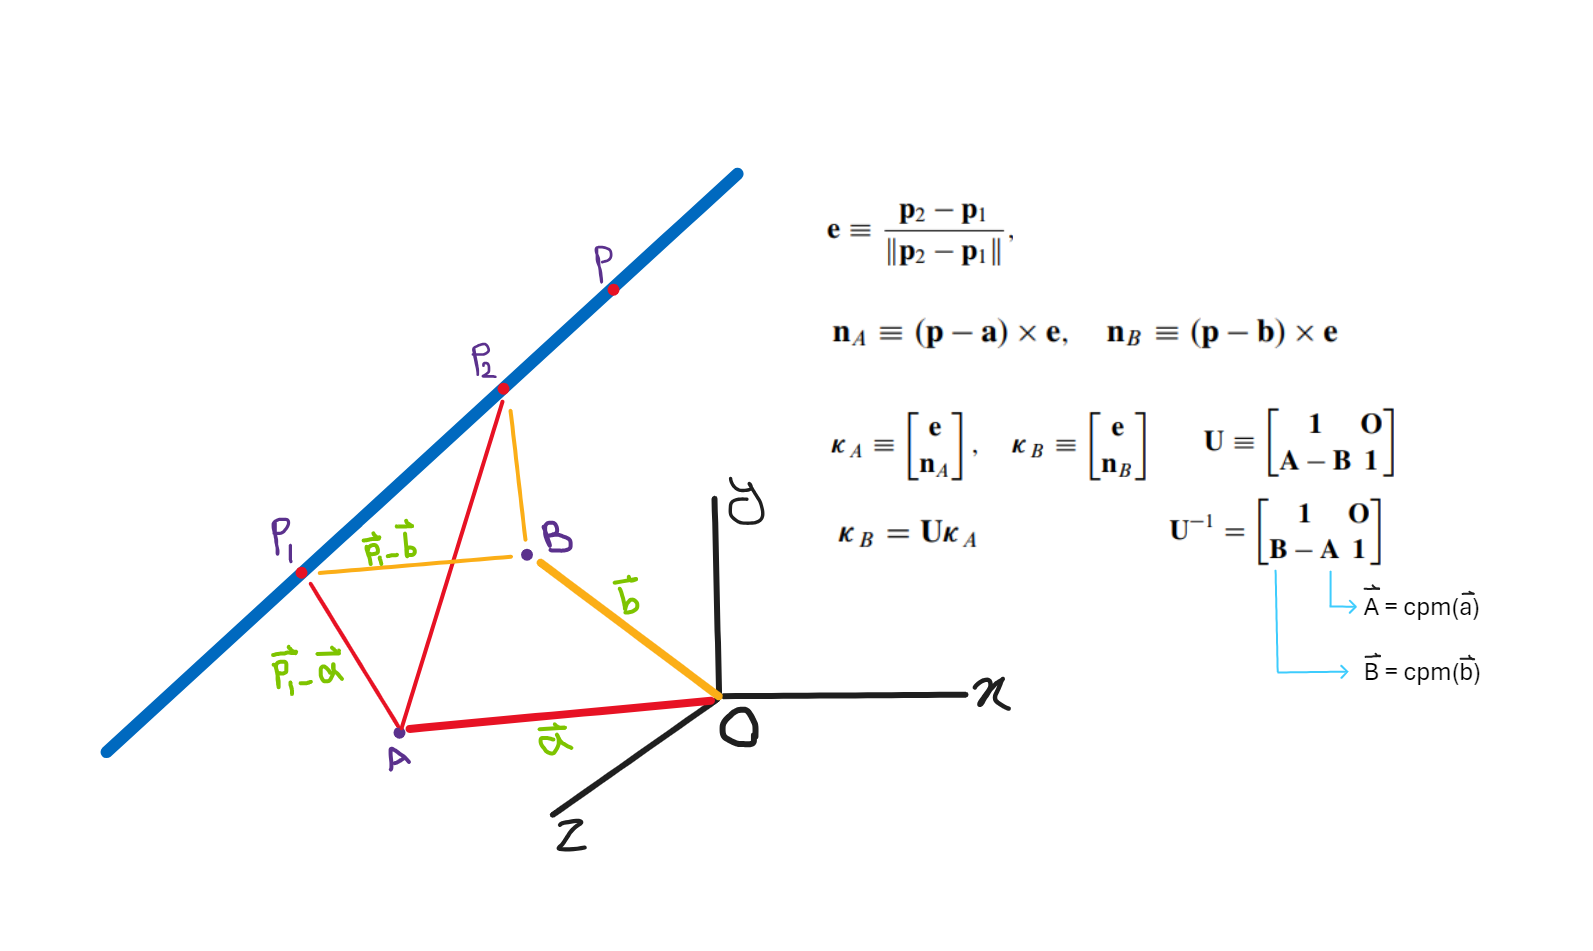
\includegraphics[width=0.5\textwidth]{P6_image.png}}
    \caption{Plucker-coordinate transfer formulas.}
    \label{fig: prob_6}
\end{figure}

The \underline{Python} code is attached to this file and also in the appendix. Here's the result of this code:
\scriptsize
\begin{verbatim}
1st Plucker line: ka = 
[[ 0.57735027]
    [ 0.57735027]
    [ 0.57735027]
    [-0.57735027]
    [ 1.15470054]
    [-0.57735027]]

2nd Plucker line: kb =
[[ 0.57735027]
    [ 0.57735027]
    [ 0.57735027]
    [ 0.        ]
    [ 0.57735027]
    [-0.57735027]]

Transformation matrix between ka & kb: U =
[[ 1.  0.  0.  0.  0.  0.]
    [ 0.  1.  0.  0.  0.  0.]
    [ 0.  0.  1.  0.  0.  0.]
    [ 0.  1.  0.  1.  0.  0.]
    [-1.  0.  0.  0.  1.  0.]
    [ 0.  0.  0.  0.  0.  1.]]

Difference of the two sides of the transformation eq:
kb = U ka -> kb - U ka =
[[0.]
    [0.]
    [0.]
    [0.]
    [0.]
    [0.]] = 0
\end{verbatim}

\vspace{10px}
\section{Problem 7: Rotation}
\subsection*{Part 1)}
Designating local coordinate system, we assume the block to rotate $\alpha = 30^\circ$ about the z-axis and then, $\beta = 30^\circ$ about the new y-axis. From the reference text book \cite{b12}, the rotation matrix for this rotation order is introduced as below.
\begin{align}
    &\mathbf{R}_{Z'Y'X'}(\alpha, \beta, \gamma) = \\
    &\begin{bmatrix}
    \cos\alpha\cos\beta & \cos\alpha\sin\beta\sin\gamma - \sin\alpha\cos\gamma & \cos\alpha\sin\beta\cos\gamma + \sin\alpha\sin\gamma \\
    \sin\alpha\cos\beta & \sin\alpha\sin\beta\sin\gamma + \cos\alpha\cos\gamma & \sin\alpha\sin\beta\cos\gamma - \cos\alpha\sin\gamma \\
    -\sin\beta & \cos\beta\sin\gamma & \cos\beta\cos\gamma
\end{bmatrix} \nonumber
\end{align}

Here $\gamma = 0$, so by substitution of values, we'll have:
\begin{align}
    \mathbf{R}_{Z'Y'}(\alpha, \beta) &= 
    \begin{bmatrix}
        \cos 30^\circ \cdot \cos 30^\circ & -\sin 30^\circ & \cos 30^\circ \cdot \sin 30^\circ \\
        \sin 30^\circ \cdot \cos 30^\circ & \cos 30^\circ & \sin 30^\circ \cdot \sin 30^\circ \\
        -\sin 30^\circ & 0 & \cos 30^\circ
    \end{bmatrix} \nonumber \\
    & = 
    \begin{bmatrix}
        0.75 & -0.5 & \frac{\sqrt{3}}{4} \\
        \frac{\sqrt{3}}{4} & \frac{\sqrt{3}}{2} & 0.25 \\
        -0.5 & 0 & \frac{\sqrt{3}}{2}
    \end{bmatrix}
\end{align}
    
\subsection*{Part 2)}
Angle of rotation:
\begin{align}
    &\phi = \cos ^{-1} \left(\frac{tr(\mathbf{R}) - 1}{2}\right) = \cos ^{-1} \left(\frac{(0.75 + \frac{\sqrt{3}}{2} \times 2) - 1}{2}\right) = 42.18^\circ
\end{align}
    
Axis of rotation:

\begin{align}
&\text{vect}(\mathbf{R}) = \frac{1}{2} 
\begin{bmatrix}
    0 - 0.25 \\
    \frac{\sqrt{3}}{4} - (-0.5) \\
    \frac{\sqrt{3}}{4} - (-0.5)
\end{bmatrix} = 
\frac{1}{2} 
\begin{bmatrix}
    - 0.125 \\
    0.4665 \\
    0.4665
\end{bmatrix} \\
&\mathbf{e} = \frac{\text{vect}(\mathbf{R})}{\sin \phi} = \frac{1}{\sin 42.18^\circ} \times
    \begin{bmatrix}
    - 0.125 \\
    0.4665 \\
    0.4665
\end{bmatrix} = 
\begin{bmatrix}
    -0.1862 \\
    0.6947 \\
    0.6947
\end{bmatrix}
\end{align}

\vspace{10px}

\section{Problem 8: Rotation of a Rigid Body}
\subsection*{Parts 1 and 3)}
Quadratic invariants of rotations are mathematical expressions that remain constant under rotations. In the context of 3D rotations, the quadratic invariants are related to the properties of rotation matrices and quaternions. These invariants are valuable in various applications, including computer graphics, robotics, and physics. Here are two primary quadratic invariants associated with rotations:
\begin{enumerate}
    \item \textbf{Trace of the Rotation Matrix}:
    \begin{itemize}
        \item For a 3x3 rotation matrix \(R\), the trace is given by \(\text{tr}(R) = R_{11} + R_{22} + R_{33}\).
        \item The trace is a quadratic invariant under rotations. For a proper (rotation) matrix, the trace is always in the range \([-1, 3]\), and its value remains constant during rotations.
    \end{itemize}
    \item \textbf{Quaternion Norm}:
    \begin{itemize}
        \item For a unit quaternion \(q = (q_0, q_1, q_2, q_3)\), the quaternion norm is given by \(\|q\|^2 = q_0^2 + q_1^2 + q_2^2 + q_3^2\).
        \item The quaternion norm is a quadratic invariant under rotations. For a unit quaternion representing a rotation, the norm is always equal to 1, and its value remains constant during rotations.
    \end{itemize}
\end{enumerate}

These quadratic invariants are useful in various algorithms involving rotations. They provide a way to check the validity of rotation representations and can be used to ensure numerical stability in rotation-related computations. \\
In this problem, however, due to the professor's opinion, the object is to derive the \underline{Euler-Rodrigues parameters} that are referred to as \textit{quadratic invariants} in the pamphlet. A Python code is written for this purpose. The real challenge is the singularity problem that happens in \textit{part three} when trying to find the E-R parameters for \(t_3=\frac{\pi}{\alpha}\). At this moment, the angle of rotation becomes \(\pi \) \textit{radians} that causes zero division error while computing \(\mathbf{e}\). The singularity problem and available ways for handling it is stated in section 12: Problem 11 in detail. \\
Here, we use the same method as \textit{Example 2.3.10} of textbook \cite{b1}. This method states that since the given matrix is symmetric, its angle of rotation is $\pi$ and its vector linear invariant vanishes, which prevents us from finding the direction of the axis of rotation from the linear invariants. However, we can use the following equation to find the unit vector $\textbf{e}$ parallel to the axis of rotation:
$$
\mathbf{e} \mathbf{e}^T = \frac{1}{2} (\mathbf{I}+\mathbf{Q})
$$
A simple inspection of the components of the two sides of the above equation reveals that all three components of e are identical and moreover, of the same sign, but we cannot tell which sign this is. Therefore,
$$
\mathbf{e} = \pm \frac{\sqrt{3}}{3} 
\begin{bmatrix}
    1\\
    1\\
    1
\end{bmatrix}
$$
Also we know that $\phi = \pi$, hence,
$$
\textbf{r} = \textbf{e} \sin \frac{\phi}{2} = \pm \frac{\sqrt{3}}{3} 
\begin{bmatrix}
    1\\
    1\\
    1
\end{bmatrix} \, \quad , \quad \, r_0 = \cos \frac{\phi}{2} = 0
$$

The \underline{Python} code is attached to this file and also in the appendix. Here's the result of this code:

\tiny
\begin{verbatim}
part 1)
Rotation angle = phi = acos(-sin(a*t/2)**2/2 + 3*cos(a*t/2)**2/2 - 1/2) radians
Rotation axis vector = e = 
[[0.77*sin(a*t/2)*cos(a*t/2)/(0.44 - (-0.33*sin(a*t/2)**2 + cos(a*t/2)**2 - 0.33)**2)**0.5]
 [0.77*sin(a*t/2)*cos(a*t/2)/(0.44 - (-0.33*sin(a*t/2)**2 + cos(a*t/2)**2 - 0.33)**2)**0.5]
 [0.77*sin(a*t/2)*cos(a*t/2)/(0.44 - (-0.33*sin(a*t/2)**2 + cos(a*t/2)**2 - 0.33)**2)**0.5]]

Euler-Rodrigues parameters of rotation:
r0 = cos(acos(-sin(a*t/2)**2/2 + 3*cos(a*t/2)**2/2 - 1/2)/2)
r = 
[[0.77*sin(a*t/2)*sin(acos(-sin(a*t/2)**2/2 + 3*cos(a*t/2)**2/2 - 1/2)/2)*cos(a*t/2)/
    (0.44 - (-0.33*sin(a*t/2)**2 + cos(a*t/2)**2 - 0.33)**2)**0.5]
 [0.77*sin(a*t/2)*sin(acos(-sin(a*t/2)**2/2 + 3*cos(a*t/2)**2/2 - 1/2)/2)*cos(a*t/2)/
    (0.44 - (-0.33*sin(a*t/2)**2 + cos(a*t/2)**2 - 0.33)**2)**0.5]
 [0.77*sin(a*t/2)*sin(acos(-sin(a*t/2)**2/2 + 3*cos(a*t/2)**2/2 - 1/2)/2)*cos(a*t/2)/
    (0.44 - (-0.33*sin(a*t/2)**2 + cos(a*t/2)**2 - 0.33)**2)**0.5]]

part 3)
E-R parameters at t = pi/(2*a):
R0 = sqrt(2)/2
R = 
[[0.4082]
 [0.4082]
 [0.4082]]
Q:
[[1/3 1/3 - sqrt(3)/3 1/3 + sqrt(3)/3]
 [1/3 + sqrt(3)/3 1/3 1/3 - sqrt(3)/3]
 [1/3 - sqrt(3)/3 1/3 + sqrt(3)/3 1/3]]
phi = pi/2
e = Matrix([[0.5773], [0.5773], [0.5773]])

E-R parameters at t = 2*pi/a:
R0 = 1
R = 
[[0]
 [0]
 [0]]
Q:
[[1 0 0]
 [0 1 0]
 [0 0 1]]
phi = 0
e = Matrix([[nan], [nan], [nan]])

E-R parameters at t = pi/a:
R0 = 0
R = 
[[nan]
 [nan]
 [nan]]
Q:
[[-1/3 2/3 2/3]
 [2/3 -1/3 2/3]
 [2/3 2/3 -1/3]]
phi = pi
e = Matrix([[nan], [nan], [nan]])

This instance is subject to singularity and thus zero division problem.
By handling the singularity, the new E-R parameters are derived.
The unknowns of the parametric axis of rotation (e): [e0, e1, e2]
The system of equations derived to solve for the mentioned unknowns:
[e0**2 - 0.333333333333333, e0*e1 - 0.333333333333333, e0*e2 - 0.333333333333333]
There are 2 answers for axis of rotation:
    R_1:  [-0.577350269189626 -0.577350269189626 -0.577350269189626]
    R_2:  [0.577350269189626 0.577350269189626 0.577350269189626]
\end{verbatim}


\subsection*{Part 2)}
When a rigid body rotates around a fixed point and the rotation matrix $Q$ giving the orientation of the body at all times is defined by sinusoidal functions of time $t$, it implies that the rotation is harmonic or oscillatory in nature.

A physical interpretation of this rotation could be a periodic motion of the rigid body. For example:

\begin{enumerate}
    \item \textbf{Pendulum Motion}: Imagine a physical system where a rigid body is attached to a fixed point by a pendulum. The body undergoes rotational motion as it swings back and forth due to gravity. The sinusoidal nature of the rotation matrix could represent the angular displacement of the body over time.
    
    \item \textbf{Vibrations}: In certain mechanical systems, rigid bodies can undergo oscillatory motion due to vibrations. For instance, a rotor in a rotating machinery may experience sinusoidal oscillations as it rotates.
    
    \item \textbf{Wave-like Motion}: In some cases, the sinusoidal nature of the rotation matrix might represent wave-like motion. This could occur in systems like robotic arms or antennas where the rigid body undergoes periodic waving or undulating motions.
    
    \item \textbf{Harmonic Oscillations}: This could also represent harmonic oscillations observed in various physical systems such as a mass attached to a spring undergoing simple harmonic motion.
\end{enumerate}

In summary, the sinusoidal nature of the rotation matrix indicates that the rigid body undergoes periodic or oscillatory motion over time, which could have various physical interpretations depending on the specific system or application.

\vspace{12px}
\section{Problem 9: Rotation matrix properties}
This problem only has matrix calculations so its fully done with Python, utilizing NumPy package. For part one, it is proved that the given matrix is a rotation matrix by showing that ot satisfies the two principal properties of rotation matrices:
\begin{align}
    \det(\mathbf{R}) = 1 \\
    \mathbf{R}^T \mathbf{R} = \mathbf{1}
\end{align}

The axis of rotation and the angle of rotation are calculated from the equations below:
\begin{gather}
    \phi = \arccos (\frac{1 - \text{tr}(\mathbf{R})}{2}) \\
    \mathbf{e} = \frac{\text{vect}(\mathbf{R})}{\sin \phi}
\end{gather}

where tr(\textbf{Q}) and vect(\textbf{Q}) are introduced in the pamphlet. Thereafter, the \textit{Euler Parameters} are calculated from:
\begin{align}
    &\mathbf{r} = \sin \frac{\phi}{2} \mathbf{e} \\
    &r_0 = \cos \frac{\phi}{2}
\end{align}

The \underline{Python} code is attached to this file and also in the appendix. Here's the result of this code:
\scriptsize
\begin{verbatim}
part 1)
|R| = 0.9999999999999998 = 1
R^T R =
[[ 1.00000000e+00  0.00000000e+00 -1.11022302e-16]
 [ 0.00000000e+00  1.00000000e+00  0.00000000e+00]
 [-1.11022302e-16  0.00000000e+00  1.00000000e+00]] 
 = I

part 2)
Rotation angle = phi = 62.799429619838094 degrees
Rotation axis vector = e =
[[-0.67859834]
 [ 0.67859834]
 [-0.28108464]]
Magnitude of e = 0.9999999999999999 = 1

part 3)
Euler-Rodrigues parameters of rotation:
r0 = 0.8535533905932737
r =
[[-0.35355339]
 [ 0.35355339]
 [-0.14644661]]
\end{verbatim}


\section{Problem 10: Aircraft rotation calculations}
\subsection*{Part 1)}
According to the pamphlet, the rotation matrix can be obtained by:
$$
\mathbf{Q} = 
\begin{bmatrix}
    \mathbf{e_1} \cdot \mathbf{e_1}^\prime & \mathbf{e_1} \cdot \mathbf{e_2}^\prime & \mathbf{e_1} \cdot \mathbf{e_3}^\prime \\
    \mathbf{e_2} \cdot \mathbf{e_1}^\prime & \mathbf{e_2} \cdot \mathbf{e_2}^\prime & \mathbf{e_2} \cdot \mathbf{e_3}^\prime \\
    \mathbf{e_3} \cdot \mathbf{e_1}^\prime & \mathbf{e_3} \cdot \mathbf{e_2}^\prime & \mathbf{e_3} \cdot \mathbf{e_3}^\prime 
\end{bmatrix}
$$
We assume the $e_1, e_2 \text{and } e_3$ are initially the unit vector of $x, y \text{and } z$ axes respectively. By doing some algebraic manipulations like subtracting and normalizing 3 primary coordinates of points a, b and c, we can achieve vectors $\mathbf{e_1}, \mathbf{e_2} \text{and } \mathbf{e_3}$. Then, having the secondary locations of these points, we can find $\mathbf{e_1}^\prime, \mathbf{e_2}^\prime \text{and } \mathbf{e_3}^\prime$ vectors and thus, the mentioned matrix can be calculated using Python. Here's the result:
$$
\mathbf{Q} = 
\begin{bmatrix}
    0.4330127 & -0.25  & 0.8660254 \\
    0.8080127  & 0.53349365  & -0.25 \\
    -0.39951905 & 0.8080127 & 0.4330127
\end{bmatrix}
$$
This result can be verified in two ways: 
\begin{enumerate}
    \item We can either check that the obtained matrix satisfies the criteria of rotation matrix which are:
    \begin{align}
        \left|\mathbf{Q}\right| = 1 \quad , \quad \mathbf{Q}^T \mathbf{Q} = \mathbf{1}
    \end{align}
    \item Or we can check that the obtained matrix can flawlessly transform $\mathbf{e_1}, \mathbf{e_2} \text{ and } \mathbf{e_3}$ vectors to $\mathbf{e_1}^\prime, \mathbf{e_2}^\prime \text{and } \mathbf{e_3}^\prime$.
\end{enumerate}
Both of these verifications are conducted in the written program. The \underline{Python} code is attached to this file and also in the appendix. Here's the result of this code:

\scriptsize
\begin{verbatim}
    Part 1:
    e1 = [1. 0. 0.], e2 = [0. 1. 0.], e3 = [0. 0. 1.]
     e1' = [ 0.4330127   0.8080127  -0.39951905],
     e2' = [-0.25        0.53349365  0.8080127 ],
     e3' = [ 0.8660254 -0.25       0.4330127]

    Roation Matrix:
    [[ 0.4330127  -0.25        0.8660254 ]
     [ 0.8080127   0.53349365 -0.25      ]
     [-0.39951905  0.8080127   0.4330127 ]]

    |Q| = 1.0000000000000002 = 1
    Q^T * Q =
    [[ 1. -0. -0.]
     [-0.  1.  0.]
     [-0.  0.  1.]] = I

    e1' - Q*e1 = [0. 0. 0.]
    e2' - Q*e2 = [0. 0. 0.]
    e3' - Q*e3 = [0. 0. 0.]
\end{verbatim}
    

\subsection*{Part 2)}
From the reference text book \cite{b12}, the rotation matrix for a local origin system that implies to rotating $\psi$ degrees about $x$, $\theta$ degrees about $y$, and $\phi$ degrees about $z$ axes is introduced as below. Note that with this deceleration, the $\mathbf{R_{x'y'z'}}$ implies to the \textit{general expression of the matrix of global rotation} as a function of $\psi$, $\theta$ and $\phi$ which imply to the \textit{triplet of Euler Angles} wanted in part 3.
\begin{align}
    &R_{x'y'z'}(\psi, \theta, \phi) = \\
    &\begin{bmatrix}
        \cos \theta \cos \phi & - \cos \theta \sin \phi & \sin \theta \\
        \sin \psi \sin \theta \cos \phi + \cos \psi \sin \phi & - \sin \psi \sin \theta \sin \phi + \cos \psi \cos \phi & -\sin \psi \cos \theta \\
        -\cos \psi \sin \theta \cos \phi & \cos \psi \sin \theta \sin \phi + \sin \psi \cos \phi & \cos \psi \cos \theta \nonumber
    \end{bmatrix}
\end{align}

\subsection*{Part 3)}
The numerical value of the rotation matrix was denoted in \textit{Part 1}; by comparing the corresponding entries in the general expression of the matrix denoted in \textit{part 2}, we find:

\begin{align}
    &\sin \theta = 0.8660254 \rightarrow \theta = 60^\circ , 120^\circ \\
    \, \nonumber \\
    \hline
    \, \nonumber \\
    &-\cos \theta \sin \phi = -\frac{1}{4} \\
    &\cos \theta \cos \phi = 0.4330127 \\
    &\rightarrow \text{for } \theta = 60^\circ : \sin \phi = \frac{1}{2} \, \& \cos \phi = 0.8660254 \nonumber \\
    &\rightarrow \phi = \text{atan2}(\frac{1}{2}, \frac{\sqrt{3}}{2}) = 30^\circ \\
    &\rightarrow \text{for } \theta = 120^\circ : \sin \phi = -\frac{1}{2} \, \& \cos \phi = -\frac{\sqrt{3}}{2} \nonumber \\
    &\rightarrow \phi = \text{atan2}(-\frac{1}{2}, \frac{-\sqrt{3}}{2}) = -150^\circ \\
    \, \nonumber \\
    \hline
    \, \nonumber \\
    &-\sin \psi \cos \theta = -\frac{1}{4} \\
    &\cos \psi \cos \theta = 0.4330127 \\
    &\rightarrow \text{for } \theta = 60^\circ : \sin \psi = \frac{1}{2} \, \& \cos \psi = \frac{\sqrt{3}}{2} \nonumber \\
    &\rightarrow \psi = \text{atan2}(\frac{1}{2}, \frac{\sqrt{3}}{2}) = 30^\circ \\
    &\rightarrow \text{for } \theta = 120^\circ : \sin \psi = -\frac{1}{2} \, \& \cos \psi = -\frac{\sqrt{3}}{2} \nonumber \\
    &\rightarrow \psi = \text{atan2}(-\frac{1}{2}, \frac{-\sqrt{3}}{2}) = -150^\circ \\
    \, \nonumber \\
    \hline
    \, \nonumber
\end{align}

Answers = 
$
\begin{cases}
    \theta = 60^\circ & \psi = 30^\circ \quad \quad \,\, \phi = 30^\circ \\
    \\
    \theta = 120^\circ & \psi = -150^\circ \quad \phi = -150^\circ 
\end{cases}
$

\vspace{1cm}

\subsection*{Part 4)}
As mentioned in \textit{part 1}, the secondary vector $\mathbf{e_4}^\prime$ can be achieved by:
\begin{align}
    \mathbf{e_4}^\prime = \mathbf{Q} \mathbf{e_4}
\end{align}
By subtracting coordinates of point \textit{d} from that of the center point of the line between \textit{b} and \textit{c}, the $\mathbf{e_4}$ vector is first normalized and the achieved as:
$$
\mathbf{e_4} = \begin{bmatrix}
    0 & 0.9701425 & 0.24253563
\end{bmatrix}
$$
Then,
\begin{align}
    \mathbf{e_4}^\prime = \mathbf{Q} \mathbf{e_4} = 
    \begin{bmatrix}
        -0.03249361 \\
        0.45693096 \\
        0.88890847
    \end{bmatrix}
\end{align}
By reversing the operation used to find $\mathbf{e_4}$ from points \textit{b}, \textit{c}, and \textit{d}, now we can find point \textit{d'} since we already have points \textit{b'} and \textit{c'}. Note that the magnitude (norm) of both $\mathbf{e_4}$ and $\mathbf{e_4}^\prime$ is equal to one. Here's the result of the Python code for this part:

\scriptsize
\begin{verbatim}
Part 4 (Bonus):
e4 = [0.         0.9701425  0.24253563]
e4' = Q * e4 =
[[-0.03249361]
 [ 0.45693096]
 [ 0.88890847]]

d' =
[[  99.73205081]
 [1003.76794919]
 [ 407.33012702]]

The e4' vector obtained using new d' =
[[-0.03249361]
 [ 0.45693096]
 [ 0.88890847]] = previously achieved e4' vector.
\end{verbatim}




\section{Problem 11: Rotation matrices}
\subsection*{Parts 1, 2 and 3)}
As for problems 6, 8 and 9, we use \textit{numpy} package from \textit{Python} to obtain the required rotation matrix parameters. The program simply implements the equations for rotation matrix parameters given in chapters 2.3.3, 2.3.4 and 2.3.6 of the textbook \cite{b1}. Then the program provides a pre-defined rotation matrix as a test and prints the results. The \underline{Python} code is attached to this file and also in the appendix. Here's the result of this code:
\scriptsize
\begin{verbatim}
    part 1: Natural invariants of rotation
    phi = 62.799429619838094 degrees
    e =
    [[-0.67859834]
     [ 0.67859834]
     [-0.28108464]]

    part 2: Linear invariants of rotation
    q0 = 0.4571067811865474
    q =
    [[-0.60355339]
     [ 0.60355339]
     [-0.25      ]]

    part 3: Euler-Rodrigues parameters of rotation
    r0 = 0.8535533905932737
    r =
    [[-0.35355339]
     [ 0.35355339]
     [-0.14644661]]
\end{verbatim}

\subsection*{Part 4)}
In the context of robotics and rotation representations, the Euler-Rodrigues representation, also known as the axis-angle representation, uses a three-dimensional vector to represent the axis of rotation and an angle to represent the amount of rotation around that axis. This representation is commonly used to describe 3D rotations.

\vspace{10px}
\subsubsection{Singularity Problem}
A singularity in the Euler-Rodrigues representation occurs when the rotation angle is exactly 180 degrees (\(\pi\) radians). At this point, the representation becomes problematic for several reasons:

\begin{enumerate}
  \item \textbf{Ambiguity of Rotation Axis:}
    \begin{itemize}
      \item When the rotation angle is 180 degrees, the axis of rotation becomes ambiguous. Any vector pointing in the same direction can be considered as the rotation axis, leading to multiple representations for the same rotation.
      \item This ambiguity is known as the "gimbal lock" problem, and it makes it challenging to uniquely recover the original rotation.
    \end{itemize}
  
  \item \textbf{Numerical Instability:}
    \begin{itemize}
      \item Numerical stability becomes an issue when the rotation angle approaches 180 degrees. Small numerical errors in the representation or computation can lead to large errors in the result.
      \item This instability can affect algorithms that involve rotations, such as interpolation or inverse kinematics.
    \end{itemize}

  \item \textbf{Loss of Degrees of Freedom:}
    \begin{itemize}
      \item In practical terms, at a 180-degree rotation, two of the three rotational degrees of freedom become aligned, causing a loss of one degree of freedom.
      \item This loss of degrees of freedom can make it difficult to smoothly interpolate between different orientations or control the robot's orientation accurately.
    \end{itemize}
\end{enumerate}

To mitigate these issues, alternative representations like quaternions are often preferred in robotics applications. Quaternions do not suffer from gimbal lock and provide a more stable representation for interpolation and numerical computations. However, it's essential to choose a representation that suits the specific requirements and constraints of the robotic system in question.

\vspace{10px}
\subsubsection{Quaternion}

A quaternion is typically represented as:
\[ q = a + bi + cj + dk \]
or in the scalar-vector form:
\[ q = (a, \mathbf{v}) \]
where $a$, $b$, $c$, and $d$ are real numbers, and $i$, $j$, and $k$ are imaginary units satisfying the following relations:
\[ i^2 = j^2 = k^2 = ijk = -1 \]

\vspace{10px}
\subsubsection{Quaternion Rotation Representation}

The quaternion representation of a rotation is defined as:
\[ q = \cos\left(\frac{\theta}{2}\right) + \sin\left(\frac{\theta}{2}\right) \mathbf{v} \]
where $\theta$ is the rotation angle, and $\mathbf{v}$ is a unit vector representing the rotation axis.

\vspace{10px}
\subsubsection{Quaternion Product}

The product of two quaternions $p = (p_0, \mathbf{p})$ and $q = (q_0, \mathbf{q})$ is computed as:
\[ pq = (p_0q_0 - \mathbf{p} \cdot \mathbf{q}, p_0\mathbf{q} + q_0\mathbf{p} + \mathbf{p} \times \mathbf{q}) \]

\vspace{10px}
\subsubsection{Conversion to Rotation Matrix}

To convert a quaternion back to a rotation matrix $R$, use the following components:
\[ R = \begin{bmatrix}
    1 - 2(q_2^2 + q_3^2) & 2(q_1q_2 - q_0q_3) & 2(q_0q_2 + q_1q_3) \\
    2(q_1q_2 + q_0q_3) & 1 - 2(q_1^2 + q_3^2) & 2(q_2q_3 - q_0q_1) \\
    2(q_1q_3 - q_0q_2) & 2(q_0q_1 + q_2q_3) & 1 - 2(q_1^2 + q_2^2)
\end{bmatrix} \]

Quaternions provide advantages in numerical stability, efficient interpolation, and avoiding gimbal lock. They are commonly used in computer graphics, robotics, and physics simulations.

\vspace{10px}
\subsubsection{Conversion of E-R parameters to R-M}
It is vital to note that the \underline{linear invariants} can be readily derived from the matrix representation of the rotation involved by simple additions and subtractions; while the \underline{Euler-Rodrigues parameters} require square roots and entail sign ambiguities. However, the former fail to produce information on the axis of rotation whenever the angle of rotation is $\pi$, whereas the latter produce that information \textit{for any value of the angle of rotation} \cite{b1}.
The Euler-Rodrigues parameters are nothing but the quaternions invented by Sir William Rowan Hamilton (1844) \cite{b13}. The Euler-Rodrigues formula for converting axis-angle representation to a rotation matrix is as follows:

R is constructed as:
$$
\begin{bmatrix}
    txx + c & txy - sz & txz + sy \\
    txy + sz & tyy + c & tyz - sx \\
    txz - sy & tyz + sx & tzz + c
\end{bmatrix}
$$
where \(c = \cos(\theta)\), \(s = \sin(\theta)\), and \(t = 1 - \cos(\theta)\). The components \(x\), \(y\), and \(z\) are the coordinates of the normalized rotation axis.

In the provided code for this section, an attempt is made to handle singularities by checking if the norm of the rotation axis is close to zero. If the norm is close to zero, it indicates that the rotation axis is nearly parallel to one of the coordinate axes, which can lead to gimbal lock. The function defined in this part gets the axis of rotation $(\mathbf{r})$ and the angle of rotation $\phi$ which is a sort of representing $(r_0)$ as inputs. Two cases are used to test the functionality of the program. Afterwards, a third test case is used to validate the way the program validates the singularities. For this purpose, an already solved problem, \textit{Example 2.3.10} of textbook \cite{b1}, is used which for input, introduces the rotation matrix as:
$$
\frac{1}{3} \times
\begin{bmatrix}
    -1 & 2 & 2 \\
    2 & -1 & 2 \\
    2 & 2 & -1
\end{bmatrix}
$$

And as output, finds:
$$
\phi = \pi \, \quad , \quad \,
\mathbf{r} = \pm \frac{\sqrt{3}}{3} \times
\begin{bmatrix}
    1 \\
    1 \\
    1
\end{bmatrix}
$$

With a short glance of the results obtained from the code, as shown below, it can be seen that the result of case (c) \_which is 3 times the calculated rotation matrix\_ fits the initial R-M of the example well.

\scriptsize
\begin{verbatim}
part 4 (Bonus):
Rotation Matrix for Case (a):
[[ 1.0000000e+00  0.0000000e+00  0.0000000e+00]
    [ 0.0000000e+00 -1.0000000e+00 -1.2246468e-16]
    [ 0.0000000e+00  1.2246468e-16 -1.0000000e+00]]

Rotation Matrix for Case (b):
[[ 0.70710678  0.          0.70710678]
    [ 0.          1.          0.        ]
    [-0.70710678  0.          0.70710678]]

Rotation Matrix for Case (c):
[[-1.  2.  2.]
    [ 2. -1.  2.]
    [ 2. -1.  2.]
    [ 2.  2. -1.]]
\end{verbatim}




\section{Appendix}
\subsection{Python code for problem 4.2)}

\begin{lstlisting}[language=Python]
import sympy as sp
from numpy import *

u, v = [], []
for i in range(3):
    u.append([sp.Symbol(f'u{i}')])
    v.append([sp.Symbol(f'v{i}')])
print('Vector U:', u)
print('Vector V:', v)

u = array(u)
v = array(v)

lhs = eye(3) + u*v.T
lhs = sp.Matrix(lhs)
LHS = lhs.det()
RHS = 1 + dot(u.T, v)
print('Left Hand Side of the equation:\t', LHS)
print('Right Hand Side of the equation:\t', RHS)
print('The difference of LHS and RHS of the equation:\t', LHS - RHS)
\end{lstlisting}
% --------------------------------------

\subsection{Python code for problem 6)}

\begin{lstlisting}[language=Python]
from numpy import *

# points on the line
P = array([[1], [2], [3]])
Q = array([[4], [5], [6]])

# two points from which the Plucker line is seen
a = array([[0], [0], [0]])
b = array([[0], [0], [1]])

# unit vector of the line passing P & Q
e = (Q - P) / linalg.norm((Q - P))

# the moments of Plucker line using point P on the
# line and two origins a & b
na = cross((P - a).flatten(), e.flatten())
nb = cross((P - b).flatten(), e.flatten())

n_a = na.reshape((3, 1))
n_b = nb.reshape((3, 1))

# Plucker line representations consisting of e & ka or kb
ka = vstack((e, n_a))
kb = vstack((e, n_b))

a = a.flatten()
b = b.flatten()

# the Cross Product Matrix (CPM) or cross product
# skew-symmetric matrix of points a & b
A = array([[0, -a[2], a[1]],
            [a[2], 0, -a[0]],
            [-a[1], a[0], 0]])

B = array([[0, -b[2], b[1]],
            [b[2], 0, -b[0]],
            [-b[1], b[0], 0]])

I = eye(3, 3)
O = zeros((3, 3))

# the transformation matrix to convert ka to kb
U = block([[I, O],
            [A - B, I]])

print(f'1st Plucker line: ka = \n{ka}\n')
print(f'2nd Plucker line: kb = \n{kb}\n')
print(f'Transformation matrix between ka & kb: U = \n{U}\n')
print('Difference of the two sides of the transformation eq:')
print(f'kb = U ka -> kb - U ka = \n{kb - U@ka} = 0')    
\end{lstlisting}
% --------------------------------------

\subsection{Python code for problem 8)}

\begin{lstlisting}[language=Python]
from sympy import *
from fractions import Fraction
from numpy import array, eye

# defining a text style class to highlight the results
class TextStyle:
    BOLD = '\033[1;34m'
    END = '\033[0m'


# defining variables and constants to abbreviate rotation matrix terms
t, alpha = symbols('t, a')
c = cos(alpha * t/2)
s = sin(alpha * t/2)
r = (2*sqrt(3)/3) * s * c
a = Fraction(1, 3)
b = Fraction(2, 3)

# given rotation matrix
Q = Matrix([
    [c**2-a*s**2, b*s**2-r, b*s**2+r],
    [b*s**2+r, c**2-a*s**2, b*s**2-r],
    [b*s**2-r, b*s**2+r, c**2-a*s**2]
])

# part 1)
print('part 1)')
vect_Q = 1/2 * Matrix([
    [Q[2, 1]-Q[1, 2]],
    [Q[0, 2]-Q[2, 0]],
    [Q[1, 0]-Q[0, 1]]
])

phi = acos((trace(Q) - 1)/2)
e = vect_Q / sin(phi)
print(f'Rotation angle = phi = {phi.evalf(2)} radians')
print('Rotation axis vector = e = ')
print(matrix2numpy(e.evalf(2)))
# pprint(e.evalf(2))

r0 = cos(phi/2)
r = sin(phi/2)*e
print('\nEuler-Rodrigues parameters of rotation:')
print(f'r0 = {r0.evalf(2)}')
print(f'r = \n{matrix2numpy(r.evalf(2))}')
# pprint(r.evalf(2))


# part 3)
print('\npart 3)')
times = [pi/2/alpha, 2*pi/alpha, pi/alpha]


def singularity_handler(Q, theta):
    # defining parametric axis of rotation (e)
    R_axis = []
    for i in range(3):
        R_axis.append([Symbol(f'e{i}')])

    E = array(R_axis)
    lhs = E@E.T  # left-hand-side of the equation
    rhs = 1/2 * (eye(3, 3) + Q)  # right-hand-side of the equation
    eq = []  # defining the system of 3 equations and 3 unknowns
    for col in range(3):
        eq.append(lhs[0][col] - rhs[0][col])

    # convert R_axis from numpy-array type to list
    R_list = array(R_axis).flatten().tolist()
    print(f'The unknowns of the parametric axis of rotation (e): {R_list}')
    print(
        f'The system of equations derived to solve for the mentioned unknowns: \n{eq}')
    ans = solve(eq, R_list)
    R_1 = sin(theta/2) * array(ans[0])
    R_2 = sin(theta/2) * array(ans[1])
    print('There are 2 answers for axis of rotation:')
    print(TextStyle.BOLD, end='')
    print(f'  R_1:  {R_1}')
    print(f'  R_2:  {R_2}')
    print(TextStyle.END, end='')


for T in times:
    # qp, rp = substituter(T)
    # vect_q = vect_Q.subs(t, T)
    # Phi = acos((trace(q) - 1)/2)
    # E = vect_q / sin(Phi)
    # R0 = cos(Phi/2)
    # R = sin(Phi/2)*E
    q = matrix2numpy(Q.subs(t, T))
    Phi = phi.subs(t, T)
    E = e.subs(t, T)
    R0 = cos(Phi/2)
    R = matrix2numpy((sin(Phi/2)*E).evalf(4))
    print(TextStyle.BOLD, end='')
    print(f'E-R parameters at t = {T}:')
    print(f'R0 = {R0}')
    print(f'R = \n{R}')
    print(TextStyle.END, end='')
    print(f'Q: \n{q}')
    print(f'phi = {Phi}')
    print(f'e = {E.evalf(4)}\n')
    if [nan] in R:
        print('This instance is subject to singularity and thus zero division problem. \nBy handling the singularity, the new E-R parameters are derived.')
        singularity_handler(q, Phi)
\end{lstlisting}
% --------------------------------------

\subsection{Python code for problem 9)}

\begin{lstlisting}[language=Python]
from numpy import *

R = array([
    [1/sqrt(2), 0, 1/sqrt(2)],
    [-1/2, 1/sqrt(2), 1/2],
    [-1/2, -1/sqrt(2), 1/2]
])

# part 1)
print('part 1)')
print(f'|R| = {linalg.det(R)} = 1')
print(f'R^T R = \n{R.T@R} = I')

# part 2)
print('\npart 2)')
vect_R = 1/2 * array([
    [R[2][1]-R[1][2]],
    [R[0][2]-R[2][0]],
    [R[1][0]-R[0][1]]
])

phi = arccos((trace(R) - 1)/2)
e = vect_R / sin(phi)

print(f'Rotation angle = phi = {rad2deg(phi)} degrees')
print(f'Rotation axis vector = e = \n{e}')
print(f'Magnitude of e = {linalg.norm(e)} = 1')

# part 3)
print('\npart 3)')
r0 = cos(phi/2)
r = sin(phi/2)*e
print('Euler-Rodrigues parameters of rotation:')
print(f'r0 = {r0}')
print(f'r = \n{r}')
\end{lstlisting}


% --------------------------------------

\subsection{Python code for problem 10)}

\begin{lstlisting}[language=Python]
from numpy import *
from numpy import round

print('Part 1:')
a = array([
    [0],
    [10],
    [0]
])

b = array([
    [7],
    [0],
    [0]
])

c = array([
    [-7],
    [0],
    [0]
])

d = array([
    [0],
    [8],
    [2]
])

ap = 1/4 * array(
    [[390],
        [4030 - 5*sqrt(3)],
        [1615 + 10*sqrt(3)]]
)

bp = 1/8 * array(
    [[800 + 14*sqrt(3)],
        [8021 + 14*sqrt(3)],
        [3214-21*sqrt(3)]]
)

cp = 1/8 * array(
    [[800 - 14*sqrt(3)],
        [7979 - 14*sqrt(3)],
        [3186 + 21*sqrt(3)]]
)

e1 = (b - c)/linalg.norm(b - c)
e2 = (a - (b+c)/2) / linalg.norm(a - (b+c)/2)
e3 = cross(e1.flatten(), e2.flatten()).reshape((3, 1))
print(f'e1 = {e1.flatten()}, e2 = {e2.flatten()}, e3 = {e3.flatten()}')

e1p = (bp - cp)/linalg.norm(bp - cp)
e2p = (ap - (bp+cp)/2) / linalg.norm(ap - (bp+cp)/2)
e3p = cross(e1p.flatten(), e2p.flatten()).reshape((3, 1))
print(
    f' e1\' = {e1p.flatten()}, \n e2\' = {e2p.flatten()}, \n e3\' = {e3p.flatten()}')


def D(x, y):
    # abirritate dot product of 2 vectors
    return dot(x.T, y)[0, 0]


Q = array([
    [D(e1, e1p), D(e1, e2p), D(e1, e3p)],
    [D(e2, e1p), D(e2, e2p), D(e2, e3p)],
    [D(e3, e1p), D(e3, e2p), D(e3, e3p)]
])


print(f'\nRoation Matrix: \n{Q}')
print(f'\n|Q| = {linalg.det(Q)} = 1')
print(f'Q^T * Q = \n{round(Q.T @ Q, decimals=5)} = I\n')

print(f'e1\' - Q*e1 = {(e1p - Q@e1).flatten()}')
print(f'e2\' - Q*e2 = {(e2p - Q@e2).flatten()}')
print(f'e3\' - Q*e3 = {(e3p - Q@e3).flatten()}')

print('\nPart 4 (Bonus):')
e4 = (d - (b+c)/2) / linalg.norm(d - (b+c)/2)
e4p = Q@e4
print(f'e4 = {e4.flatten()}')
print(f'e4\' = Q * e4 = \n{e4p}')

dp = e4p * linalg.norm(d - (b+c)/2) + ((bp+cp)/2)

e4pp = (dp - (bp+cp)/2) / linalg.norm(dp - (bp+cp)/2)

print(f'\nd\' = \n{dp}')
print(
    f'\nThe e4\' vector obtained using new d\' = \n{e4pp} = previously achieved e4\' vector.')
\end{lstlisting}    

% --------------------------------------

\subsection{Python code for problem 11)}

\begin{lstlisting}[language=Python]
from numpy import *

def vect(R):
    vect_R = 1/2 * array([
        [R[2][1]-R[1][2]],
        [R[0][2]-R[2][0]],
        [R[1][0]-R[0][1]]
    ])
    return vect_R

def NaturalInvariant(Q):
    phi = arccos((trace(Q) - 1)/2)
    e = vect(Q) / sin(phi)
    return phi, e

def LinearInvariant(Q):
    phi, e = NaturalInvariant(Q)
    q0 = cos(phi)
    q = sin(phi)*e
    print(f'q0 = {q0}')
    print(f'q = \n{q}\n')

def EulerRodriguesPara(Q):
    phi, e = NaturalInvariant(Q)
    r0 = cos(phi/2)
    r = sin(phi/2)*e
    print(f'r0 = {r0}')
    print(f'r = \n{r}\n')

R = array([
    [1/sqrt(2), 0, 1/sqrt(2)],
    [-1/2, 1/sqrt(2), 1/2],
    [-1/2, -1/sqrt(2), 1/2]
])

print('part 1: Natural invariants of rotation')
Phi, E = NaturalInvariant(R)
print(f'phi = {rad2deg(Phi)} degrees')
print(f'e = \n{E}\n')

print('part 2: Linear invariants of rotation')
LinearInvariant(R)

print('part 3: Euler-Rodrigues parameters of rotation')
EulerRodriguesPara(R)

print('part 4 (Bonus):')

def euler_rodrigues_to_rotation_matrix(theta, axis):
    """
    Convert Euler-Rodrigues parameters to a rotation matrix.

    Parameters:
    - theta: Rotation angle in radians.
    - axis: 3D axis of rotation as a numpy array [x, y, z].

    Returns:
    - Rotation matrix as a 3x3 numpy array.
    """
    axis = asarray(axis)
    # Normalize the rotation axis to handle singularities
    axis = axis / linalg.norm(axis)

    # Extract components of the normalized rotation axis
    x, y, z = axis

    c = cos(theta)
    s = sin(theta)
    t = 1 - c

    # Build the rotation matrix
    rotation_matrix = array([
        [t*x*x + c, t*x*y - s*z, t*x*z + s*y],
        [t*x*y + s*z, t*y*y + c, t*y*z - s*x],
        [t*x*z - s*y, t*y*z + s*x, t*z*z + c]
    ])

    return rotation_matrix

# Test the function with two inputs:

# (a) Case where singularity happens
theta_a = pi  # 180 degrees
axis_a = array([1, 0, 0])
rotation_matrix_a = euler_rodrigues_to_rotation_matrix(theta_a, axis_a)

# (b) Case where singularity does not happen
theta_b = pi / 4  # 45 degrees
axis_b = array([0, 1, 0])
rotation_matrix_b = euler_rodrigues_to_rotation_matrix(theta_b, axis_b)

# (c) Case where singularity happens
theta_c = pi  # 180 degrees
axis_c = sqrt(3)/3 * array([1, 1, 1])
rotation_matrix_c = euler_rodrigues_to_rotation_matrix(theta_c, axis_c)

print("Rotation Matrix for Case (a):")
print(rotation_matrix_a)

print("\nRotation Matrix for Case (b):")
print(rotation_matrix_b)

print("\nRotation Matrix for Case (c):")
print(3*rotation_matrix_c)
\end{lstlisting}

% --------------------------------------



\begin{thebibliography}{00}

\bibitem{b1} J. Angeles, ``Fundamentals of Robotic Mechanical Systems'', Theory, Methods, and Algorithms, 4th edition, Springer.

\bibitem{b2} Z. Pandilov, V. Dukovski, ``Comparison of the Characteristics Between Serial and Parallel Robots'', Acta Tehnica Corviniensis - Bulletin of Engineering. [Online]. Available: \href{https://acta.fih.upt.ro/pdf/2014-1/ACTA-2014-1-19.pdf}{https://acta.fih.upt.ro/pdf/2014-1/ACTA-2014-1-19.pdf}

\bibitem{b3} B. Brumson, ``Parallel Kinematic Robots'', 2002. [Online]. Available: \href{https://www.automate.org/robotics/industry-insights/parallel-kinematic-robots}{https://www.automate.org/robotics/industry-insights/parallel-kinematic-robots}

\bibitem{b4} F. C. Park, ``Parallel Robots'', Springer, London, 2014. [Online]. Available: \url{https://doi.org/10.1007/978-1-4471-5102-9_174-1}

\bibitem{b5} en.wikipedia.org. \url{https://en.wikipedia.org/wiki/Nao_(robot)}

\bibitem{b6} ``NAO: Personal Robot Teaching Assistant'', SoftBank Robotics America.\, \url{https://us.softbankrobotics.com/nao}

\bibitem{b7} ``NAO the humanoid and programmable robot'', Aldebaran.\, \url{https://www.aldebaran.com/en/nao}

\bibitem{b8} ``Nao - ROBOTS: Your Guide to the World of Robotics''.\, \url{https://robotsguide.com/robots/nao/}

\bibitem{b9} M. Ceccarelli, M. Russo, (2020). ``Parallel Architectures for Humanoid Robots''. Robotics, 9(4). [Online]. Available: \url{https://doi.org/10.3390/robotics9040075}

\bibitem{b10} N. Kofinas, E. Orfanoudakis, M. G. Lagoudakis, ``Complete Analytical Forward and Inverse Kinematics for the NAO Humanoid Robot''. J Intell Robot Syst 77, (2015). [Online]. Available: \url{https://doi.org/10.1007/s10846-013-0015-4}

\bibitem{b11} ``Mechanical joint''. (2023, September 20). In Wikipedia. [Online]. Available: \url{https://en.wikipedia.org/wiki/Mechanical_joint}

\bibitem{b12} J. J. Craig, ``Introduction to Robotics'', 3d edition, Pearson Education, Inc.

\bibitem{b13} Hamilton, W.R., 1844, ``On quaternions: or a new system of imaginaries in algebra'', Phil. Mag., 3rd. ser. 25, pp. 489-495.
\end{thebibliography}


\vspace{12pt}

\section{Conclusion}
\textbf{
    In conclusion, this report has provided a comprehensive overview of several important concepts in robotics. We have explored the kinematics and dynamics of fixed-based and mobile-based robots, examined the mechanics of mechanical joints, and delved into the mathematical background necessary for understanding rotational transformations. Additionally, we have discussed the significance of yaw, pitch, and roll angles in describing the orientation of rigid bodies, as well as the properties and applications of rotation matrices. By completing the assigned problems, we have gained valuable insight into the theoretical foundations and practical implications of these concepts in the field of robotics. Moving forward, this knowledge will serve as a solid foundation for further exploration and experimentation in robotics research and development.
}
    
\end{document}
